\chapter{Implementation}
\label{chap:implementation}

\section{Introduction}
This chapter presents the technical implementation of the Tahkik platform. We begin by introducing the languages and frameworks used across all system components, then walk through the realized interfaces of both the mobile application and the web dashboard.

% ─────────────────────────────────────────────────────────────────────────────
\section{Technologies and Frameworks}
\label{sec:impl_tech}

\begin{emeraldbox}[title=Technology Stack]
The Tahkik platform is built on a modern, cross-platform stack that separates concerns across the mobile client, web dashboard, AI backend, and data layer. Each technology was chosen for its performance, community support, and fitness for the specific layer it serves.
\end{emeraldbox}

\subsection{Mobile Application — Flutter \& Dart}

\begin{figure}[H]
  \centering
  \begin{minipage}[c]{0.18\textwidth}
    \centering
    
\includegraphics[width=\linewidth]{figures/tech/flutter.png}
  \end{minipage}
  \hspace{2em}
  \begin{minipage}[c]{0.18\textwidth}
    \centering
    
\includegraphics[width=\linewidth]{figures/tech/dart.png}
  \end{minipage}
  \caption{Flutter and Dart logos}
  \label{fig:impl_flutter_dart}
\end{figure}

\textbf{Flutter} is Google's open-source UI toolkit for building natively compiled applications for mobile, web, and desktop from a single codebase. The Tahkik mobile application targets Android and iOS learners and is built entirely in Flutter, enabling consistent UI and shared business logic across both platforms.

\textbf{Dart} is the programming language underlying Flutter. Its strong typing, async/await model, and just-in-time compilation make it well suited for reactive UI development and real-time audio streaming.

\subsection{Web Dashboard — React}

\begin{figure}[H]
  \centering
  
\includegraphics[width=0.18\textwidth]{figures/tech/react.png}
  \caption{React logo}
  \label{fig:impl_react}
\end{figure}

\textbf{React} is a declarative, component-based JavaScript library developed by Meta for building user interfaces. The Tahkik Dashboard — used by teachers and administrators — is a React single-page application that communicates with Supabase directly through its client SDK and with the Go server for AI-related operations.

\subsection{Backend API — Go}

\begin{figure}[H]
  \centering
  
\includegraphics[width=0.22\textwidth]{figures/tech/golang.png}
  \caption{Go logo}
  \label{fig:impl_go}
\end{figure}

\textbf{Go} (Golang) is a statically typed, compiled language developed by Google, known for its simplicity and high concurrency performance. The Tahkik Go server acts as the orchestration layer between the mobile/web clients and the AI processing service, handling WebSocket audio streams and REST API endpoints.

\subsection{AI Server — Python \& FastAPI}

\begin{figure}[H]
  \centering
  \begin{minipage}[c]{0.18\textwidth}
    \centering
    
\includegraphics[width=\linewidth]{figures/tech/python.png}
  \end{minipage}
  \hspace{2em}
  \begin{minipage}[c]{0.25\textwidth}
    \centering
    
\includegraphics[width=\linewidth]{figures/tech/fastapi.png}
  \end{minipage}
  \caption{Python and FastAPI logos}
  \label{fig:impl_python_fastapi}
\end{figure}

\textbf{Python} is the leading language for machine learning and audio processing. The AI backend runs the OpenAI \textbf{Whisper} model, which transcribes Arabic Quran recitations, detects Tajweed errors, and returns a confidence score.

\textbf{FastAPI} is a modern, high-performance Python web framework for building APIs with automatic OpenAPI documentation. It serves as the HTTP/WebSocket interface for the Whisper inference pipeline, providing low-latency endpoints consumed by the Go server.

\subsection{Backend-as-a-Service — Supabase}

\begin{figure}[H]
  \centering
  
\includegraphics[width=0.16\textwidth]{figures/tech/supabase.png}
  \caption{Supabase logo}
  \label{fig:impl_supabase}
\end{figure}

\textbf{Supabase} is an open-source Firebase alternative built on top of PostgreSQL. It provides the Tahkik platform with:
\begin{itemize}[leftmargin=2em]
  \item \textbf{Authentication} — JWT-based email/password and Google Sign-In.
  \item \textbf{Database} — PostgreSQL with Row Level Security (RLS) policies.
  \item \textbf{Storage} — Audio file storage for submitted recitations.
  \item \textbf{Real-time} — Live subscriptions for teacher notifications.
\end{itemize}

\begin{figure}[H]
  \centering
  
\includegraphics[width=0.14\textwidth]{figures/tech/postgresql.png}
  \caption{PostgreSQL — underlying Supabase database engine}
  \label{fig:impl_postgresql}
\end{figure}

\subsection{Technology Stack Summary}

\begin{table}[H]
  \centering
  \caption{Summary of technologies used in the Tahkik platform}
  \label{tab:impl_tech_summary}
  \renewcommand{\arraystretch}{1.4}
  \begin{tabular}{llp{7cm}}
    \toprule
    \textbf{Layer} & \textbf{Technology} & \textbf{Role} \\
    \midrule
    Mobile App     & Flutter / Dart   & Cross-platform learner application (iOS \& Android) \\
    Web Dashboard  & React            & Teacher and admin web interface \\
    Backend API    & Go               & REST + WebSocket server, audio routing \\
    AI Server      & Python / FastAPI & Whisper inference, Tajweed error detection \\
    BaaS           & Supabase         & Auth, PostgreSQL DB, Storage, Real-time \\
    AI Model       & OpenAI Whisper   & Arabic speech-to-text and pronunciation scoring \\
    \bottomrule
  \end{tabular}
\end{table}

% ─────────────────────────────────────────────────────────────────────────────
\section{Mobile Application — Tahkik App}
\label{sec:impl_mobile}

\begin{emeraldbox}[title=Mobile Application]
The Tahkik mobile application is the primary interface for learners. Built with Flutter, it provides an onboarding flow, authentication screens, Quran browsing with Warsh script rendering, real-time recitation recording with WebSocket audio streaming, AI feedback visualization, and progress tracking.
\end{emeraldbox}

\subsection{Authentication Screens}

\begin{figure}[H]
  \centering
  \begin{minipage}[t]{0.42\textwidth}
    \centering
    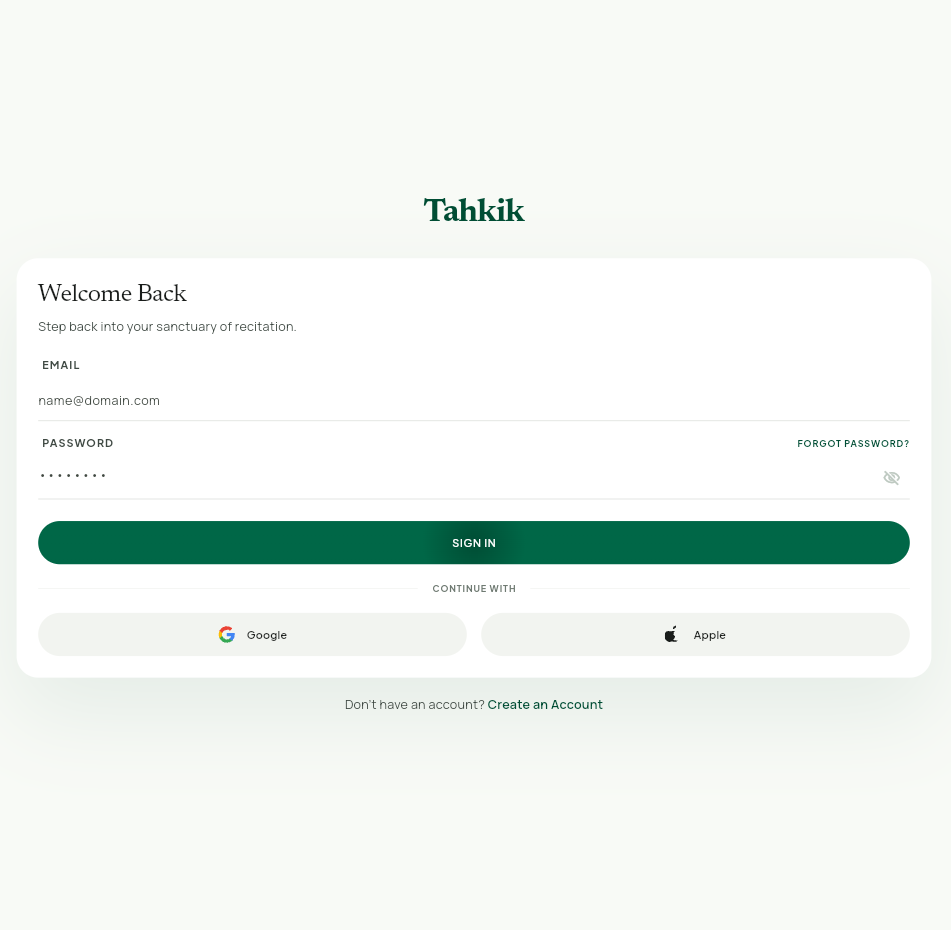
\includegraphics[width=\linewidth,height=14cm,keepaspectratio]{figures/screen_login.png}
    \caption{Login screen}
    \label{fig:impl_app_login}
  \end{minipage}
  \hspace{1.5em}
  \begin{minipage}[t]{0.42\textwidth}
    \centering
    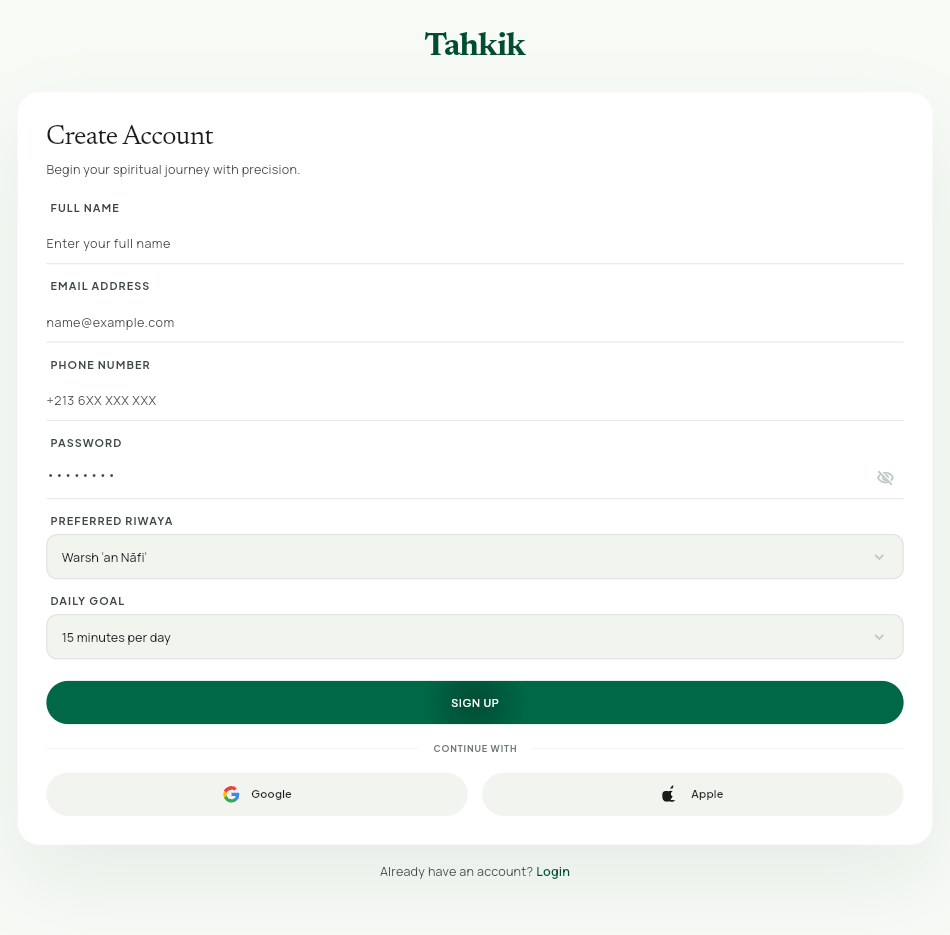
\includegraphics[width=\linewidth,height=14cm,keepaspectratio]{figures/screen_signup.png}
    \caption{Sign-up screen}
    \label{fig:impl_app_signup}
  \end{minipage}
\end{figure}

\subsection{Onboarding}

\begin{figure}[H]
  \centering
  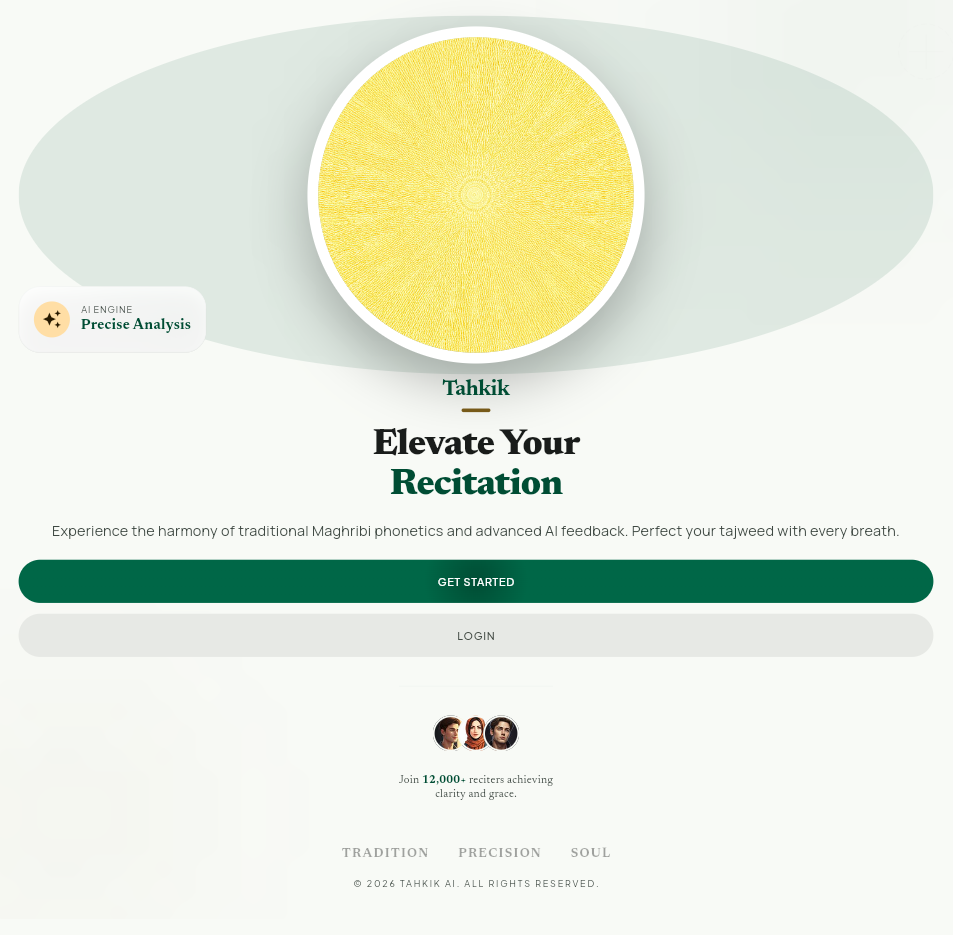
\includegraphics[width=0.5\textwidth,height=14cm,keepaspectratio]{figures/screen_onboarding.png}
  \caption{Onboarding screen — recitation preferences setup}
  \label{fig:impl_app_onboarding}
\end{figure}

\subsection{Core App Screens}

The following screens will be added upon completion of the UI polish sprint.

\begin{figure}[H]
  \centering
  \begin{minipage}[c][12cm][c]{0.42\textwidth}
    \centering
    \fbox{\parbox[c][11cm][c]{\dimexpr\linewidth-2\fboxsep-2\fboxrule}{%
      \centering\textcolor{black}{\large\textit{Screenshot to be added}}\\[0.4em]
      \textcolor{black}{\small Quran Reader}
    }}
  \end{minipage}
  \hspace{1.5em}
  \begin{minipage}[c][12cm][c]{0.42\textwidth}
    \centering
    \fbox{\parbox[c][11cm][c]{\dimexpr\linewidth-2\fboxsep-2\fboxrule}{%
      \centering\textcolor{black}{\large\textit{Screenshot to be added}}\\[0.4em]
      \textcolor{black}{\small Recitation Recording}
    }}
  \end{minipage}
  \caption{Tahkik App — Quran reader and recitation recording (coming soon)}
  \label{fig:impl_app_reader}
\end{figure}

\begin{figure}[H]
  \centering
  \begin{minipage}[c][12cm][c]{0.42\textwidth}
    \centering
    \fbox{\parbox[c][11cm][c]{\dimexpr\linewidth-2\fboxsep-2\fboxrule}{%
      \centering\textcolor{black}{\large\textit{Screenshot to be added}}\\[0.4em]
      \textcolor{black}{\small AI Feedback View}
    }}
  \end{minipage}
  \hspace{1.5em}
  \begin{minipage}[c][12cm][c]{0.42\textwidth}
    \centering
    \fbox{\parbox[c][11cm][c]{\dimexpr\linewidth-2\fboxsep-2\fboxrule}{%
      \centering\textcolor{black}{\large\textit{Screenshot to be added}}\\[0.4em]
      \textcolor{black}{\small Progress Dashboard}
    }}
  \end{minipage}
  \caption{Tahkik App — AI feedback and progress tracking (coming soon)}
  \label{fig:impl_app_feedback}
\end{figure}

% ─────────────────────────────────────────────────────────────────────────────
\section{Web Dashboard — Tahkik Dashboard}
\label{sec:impl_dashboard}

\begin{emeraldbox}[title=Web Dashboard]
The Tahkik Dashboard is a React single-page application used by teachers and administrators. Teachers can review student recitations, listen to audio submissions, consult AI-generated Tajweed error reports, and manage their student roster. Administrators have full platform oversight with analytics, user management, and AI health monitoring.
\end{emeraldbox}

\subsection{Admin Overview}

\begin{figure}[H]
  \centering
  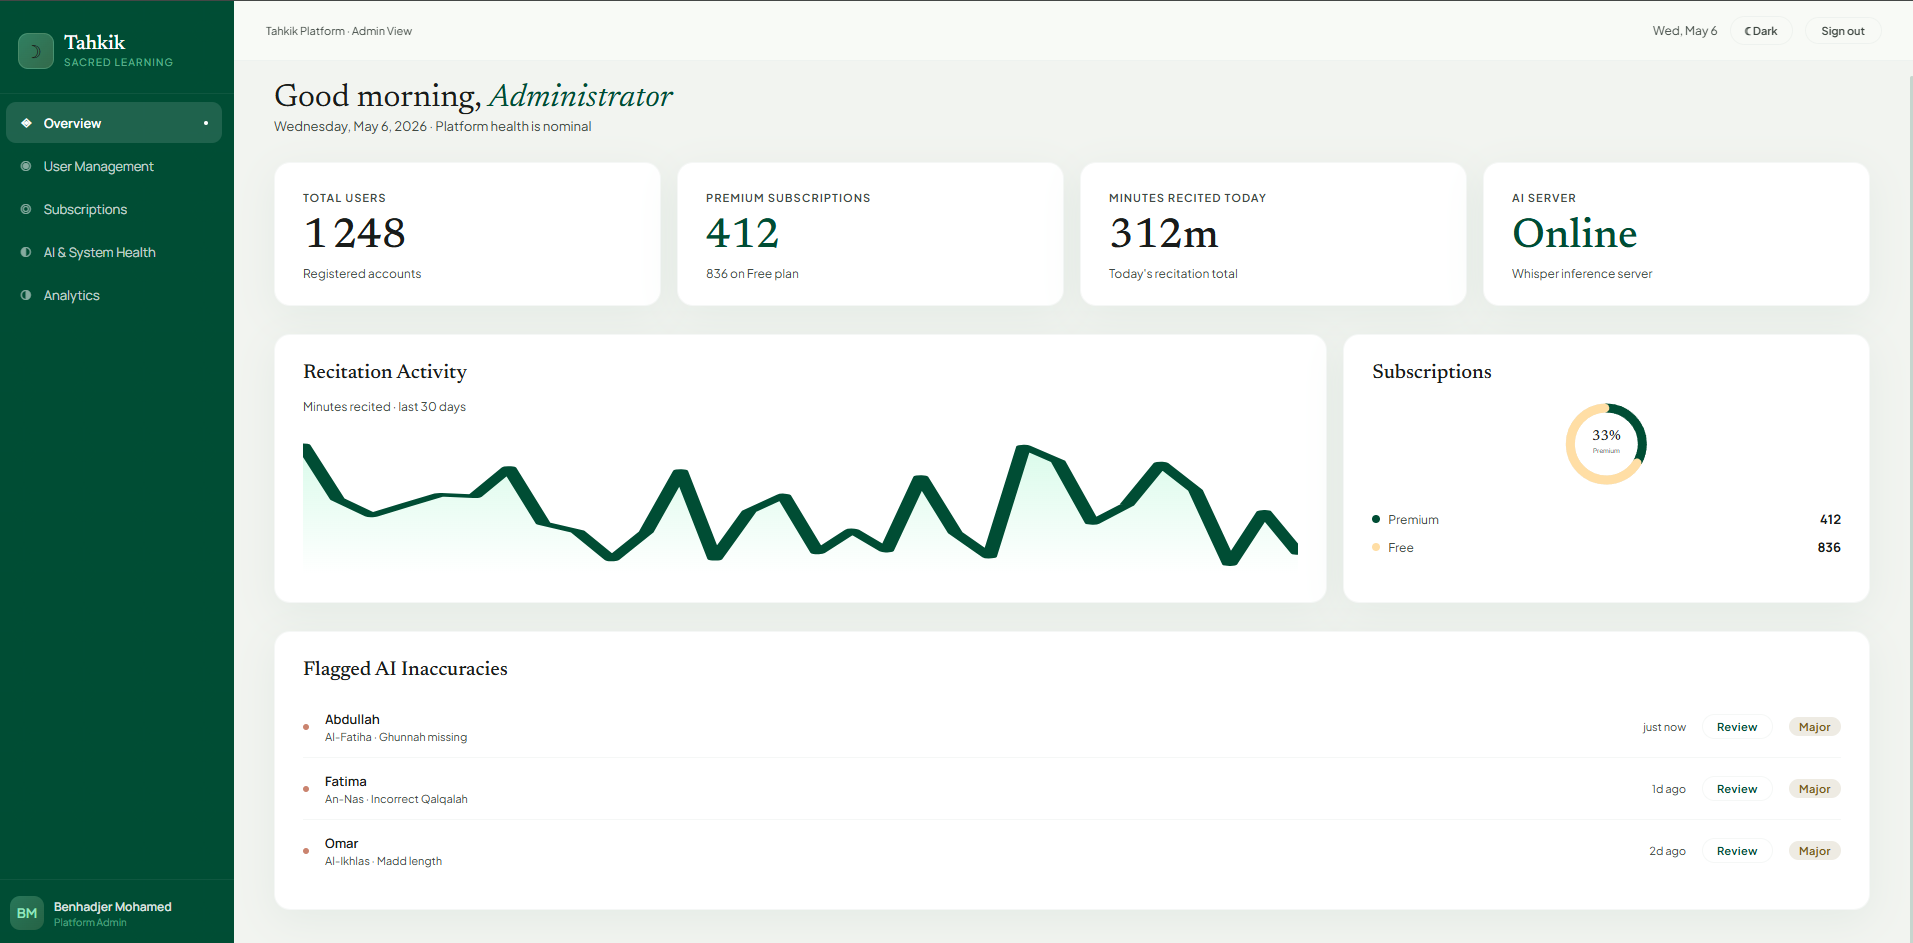
\includegraphics[width=\textwidth,height=0.55\textheight,keepaspectratio]{figures/dash_overview.png}
  \caption{Tahkik Dashboard — Admin overview with platform statistics}
  \label{fig:impl_dash_overview}
\end{figure}

\subsection{AI \& System Health}

\begin{figure}[H]
  \centering
  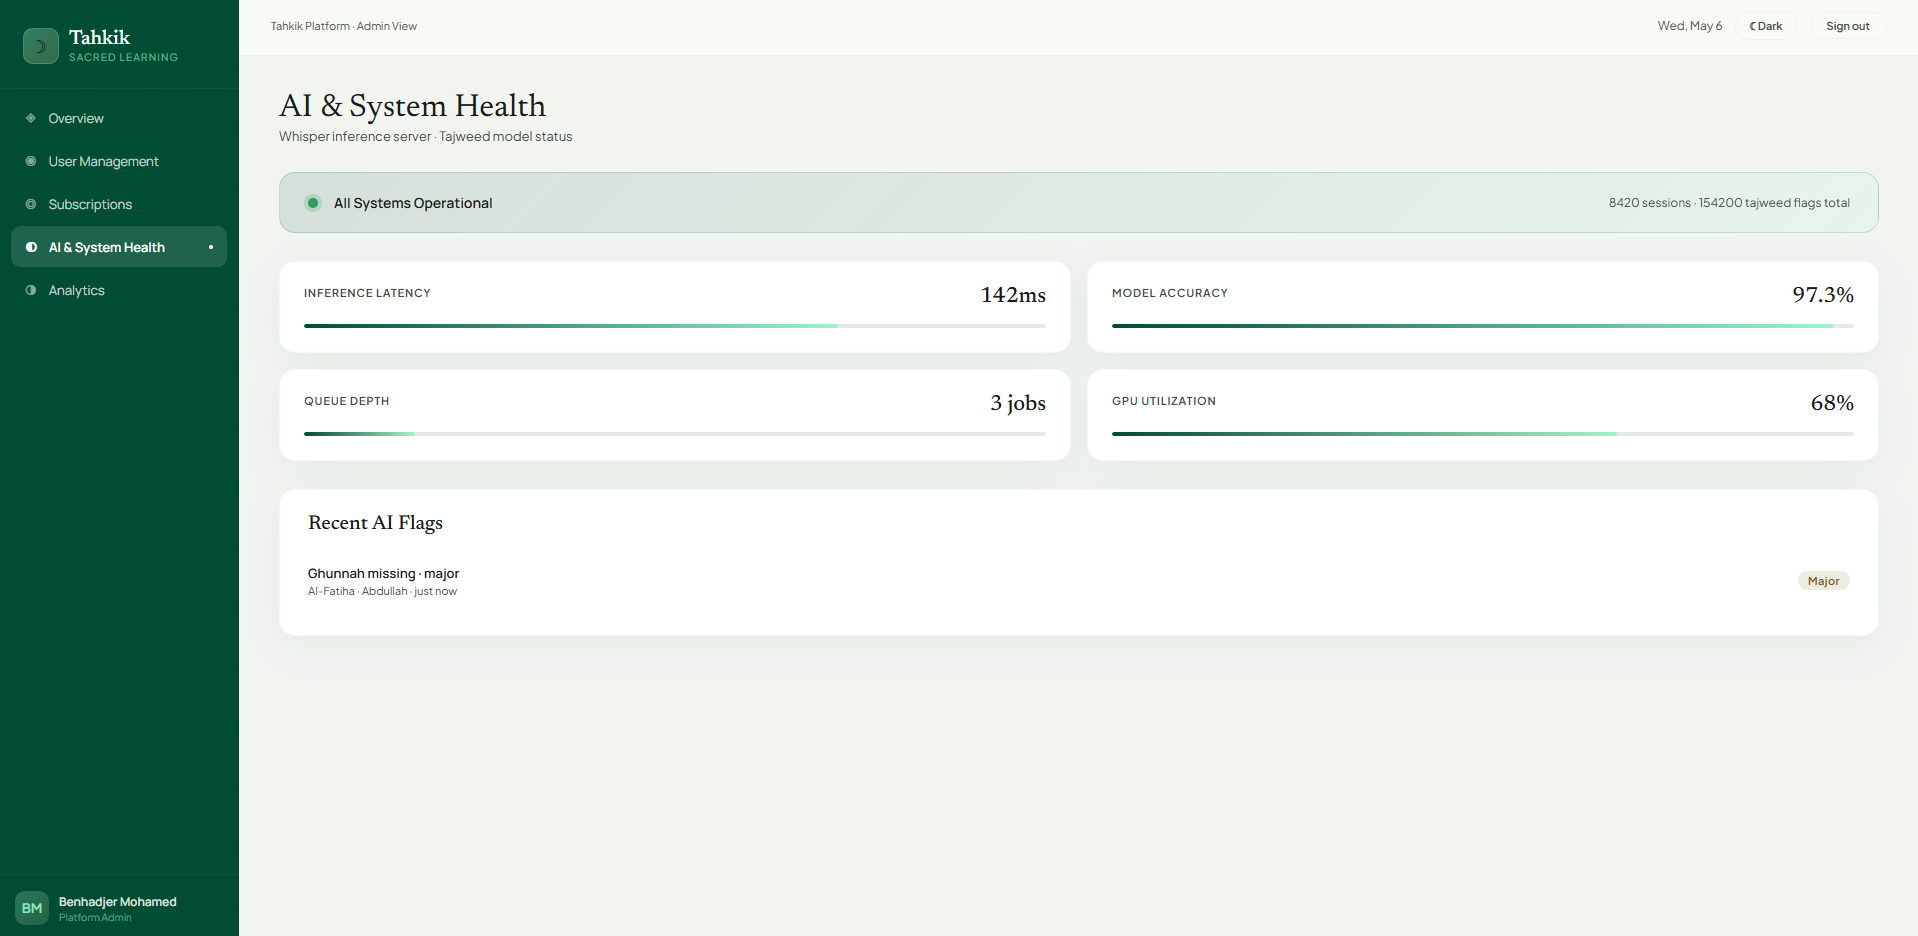
\includegraphics[width=\textwidth,height=0.55\textheight,keepaspectratio]{figures/dash_ai_health.png}
  \caption{Tahkik Dashboard — AI and system health monitoring}
  \label{fig:impl_dash_ai_health}
\end{figure}

\subsection{Recitation Review Panel}

\begin{figure}[H]
  \centering
  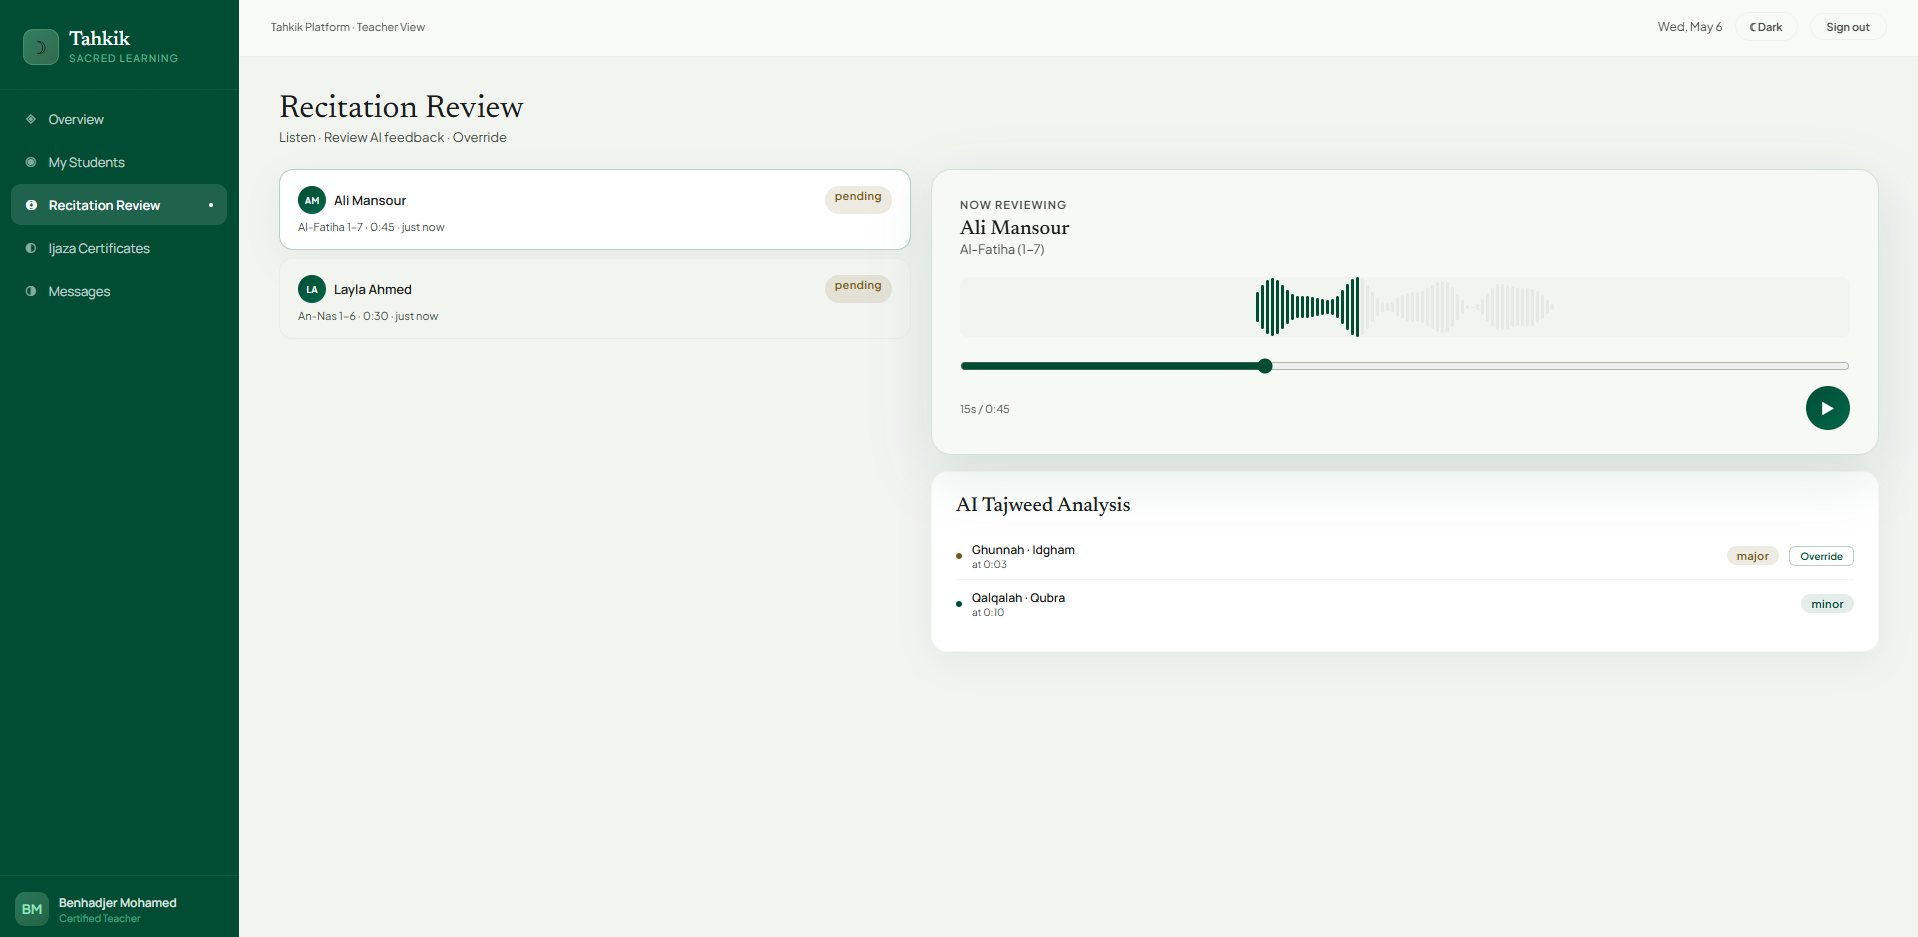
\includegraphics[width=\textwidth,height=0.55\textheight,keepaspectratio]{figures/dash_recitation_review.png}
  \caption{Tahkik Dashboard — Teacher recitation review panel}
  \label{fig:impl_dash_recitation}
\end{figure}

\subsection{Student Roster}

\begin{figure}[H]
  \centering
  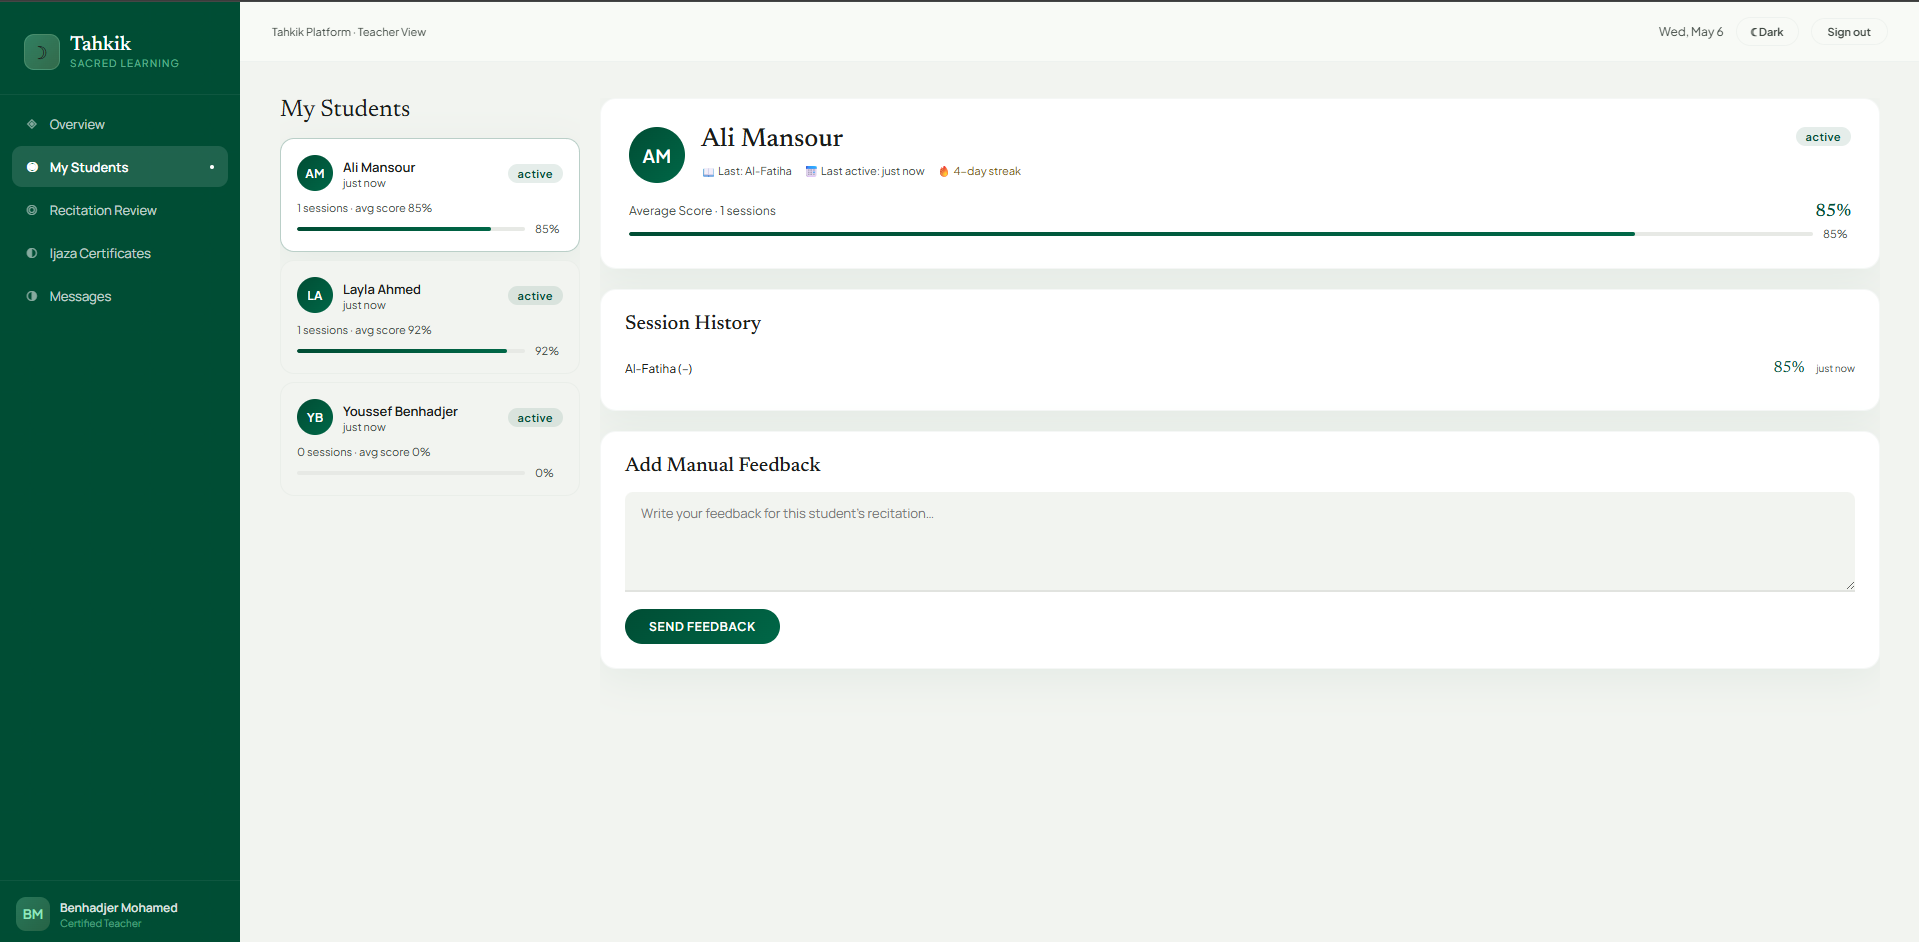
\includegraphics[width=\textwidth,height=0.55\textheight,keepaspectratio]{figures/dash_student_roster.png}
  \caption{Tahkik Dashboard — Teacher student roster}
  \label{fig:impl_dash_roster}
\end{figure}

\subsection{User Management}

\begin{figure}[H]
  \centering
  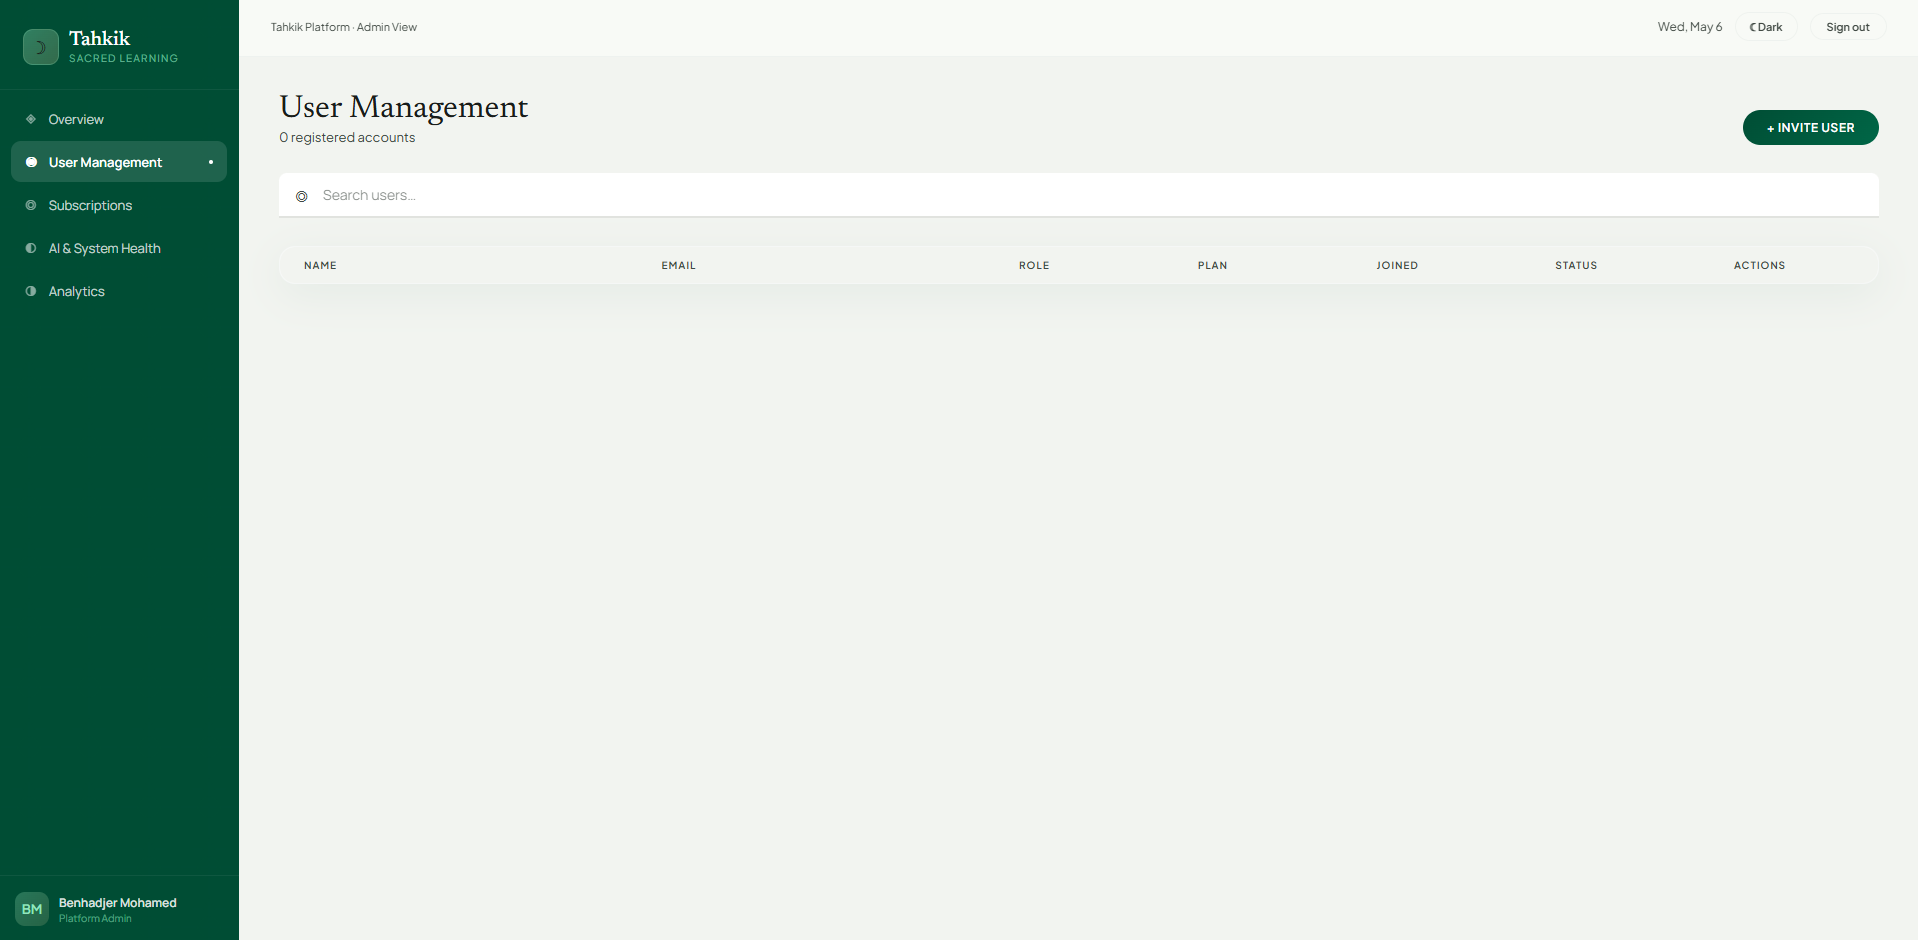
\includegraphics[width=\textwidth,height=0.55\textheight,keepaspectratio]{figures/dash_user_management.png}
  \caption{Tahkik Dashboard — Admin user management}
  \label{fig:impl_dash_users}
\end{figure}

% ─────────────────────────────────────────────────────────────────────────────
\section{Conclusion}
This chapter presented the full technology stack powering the Tahkik platform and the realized interfaces of both the mobile application and the web dashboard. Flutter and Dart deliver a smooth cross-platform mobile experience; React enables a feature-rich teacher and admin dashboard; Go and Python/FastAPI form a performant backend pipeline; and Supabase provides a robust, scalable data and authentication layer. The remaining mobile screens will be added upon completion of the final UI sprint.
